\part*{Mecânicas Universais do jogo}
\section{Mecânica}
 O jogo se inicia no último andar do campo de concentração de Belsen.O mapa será como o mostrado na figura \ref{hud}. O personagem estará em uma ala aberta no início do jogo. O objetivo de cada fase é procurar a chave que dá acesso á fase seguinte. Essa chave está em algum local aleatório das salas que são geradas de forma aleatória.O formato da chave pode mudar de uma fase para outra, mas será sempre um objeto que destrava uma porta específica em alguma sala para a fase seguinte. Toda vez que o jogador perder (for pego por um guarda ou for abatido) o mapa é carregado novamente. Na história, a justificativa para essa mecânica é que a cada vez que ele é capturado e consegue fugir novamente, ele pensa em como conseguir fugir se a estrutura for diferente.

Na seção \ref{ctrl} foi mostrado todas as formas de controlar o personagem dentro do jogo. Nos tópicos dentro dessa seção será detalhado como se dará essa interação entre o personagem e os itens.

\section{Movimentando os itens}
Os itens serão gerados de forma aleatória nas salas, logo, ocasionalmente, o jogador poderá encontrar uma cadeira ou mesa na frente da porta. Nesses casos, ao utilizar a opção de interagir com itens ('B' no joystick do XBOX 360 / K no teclado) o personagem poderá mover os objetos em cena.

\section{Itens coletáveis}
Alguns itens serão coletáveis pelo personagem, para coletá-los é só seguir os comandos descritos na seção \ref{ctrl} (Controles). Os itens serão os itens de saúde descritos na seção \ref{edmond}, a pílula e o kit médico, no caso.

Além desses itens, o personagem poderá coletar armas que estão descritos no tópico \ref{armas} que causam diferentes danos aos inimigos.

\subsection{\label{colecionaveis}{Itens colecionáveis}}
Não haverão itens colecionáveis no jogo.

\section{Inimigos}
\subsection{Guardas}

Os guardas, inimigos mais frequentes do jogo, estarão presentes no jogo desde a primeira fase e são sub-dividos em três tipos, que serão descritos nos próximos itens. São os únicos inimigos capazes de retirar uma vida do personagem, independentemente da quantidade de vida que o mesmo possua.

Os guardas estarão munidos de uma lanterna, para investigar as salas em busca de fugitivos. Uma vez que o policial avistar o personagem principal, ele emitirá um grito de ordem e, se o personagem não abater o policial em até dois segundos, o jogo congelará e uma animação mostrando mais policiais chegando para aprisionar o personagem terá início. A tela apaga e, se o personagem ainda tiver alguma vida, a partida é reiniciada e uma vida é descontada do personagem. Caso o personagem tenha perdido a última vida, a tela de \textit{Game Over} aparece.

\subsubsection*{Guarda acomodado}

O guarda acomodado finge que está trabalhando, andando de um lado para o outro, mas sempre dentro de um eixo pré-determinado (Y ou X). Faz o mesmo que o anterior ao encontrar o personagem.
\begin{figure}[h]
    \centering
    \caption{Imagem do guarda acomodado \textit{in game}}
     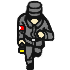
\includegraphics[keepaspectratio=true,scale=4]{images/guarda2.png}
\end{figure}

\subsubsection*{Guarda pertubado}

Completamente assustado com a atual situação, esse guarda anda em todas as direções, completamente sem rumo, em busca de algum fugitivo perdido pelas salas. Além disso, ele anda mais rápido também.
\begin{figure}[h]
    \centering
    \caption{Imagem do guarda pertubado \textit{in game}}
     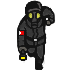
\includegraphics[keepaspectratio=true,scale=4]{images/guarda3.png}
\end{figure}

\subsection{Fantasmas}
Os fantasmas são divididos em dois grupos, os fantasmas comuns e os especiais, conforme descrito na seção \ref{characters}. Os fantasmas comuns surgirão sempre que o jogador abater um guarda durante o jogo. 

O fantasma surgirá então na posição que o guarda se encontrava antes de ser abatido. Ele irá vagar aleatoriamente pela sala, ocasionalemnte vindo ao encontro do player. 

Ao permanecer próximo ao jogador, o fantasma reduz a vida do personagem em 10\% a cada contato e 15\% da barra de sanidade.

A medida que a barra de sanidade for reduzida, a velocidade do fantasma é incrementada, o que pode aumentar o número de contatos com o player, reduzindo ainda mais a vida e a sanidade do mesmo, forçando o player a fugir daquela sala o mais rápido possível.

\begin{figure}[h]
    \centering
    \caption{Imagem do fantasma do guarda \textit{in game}}
     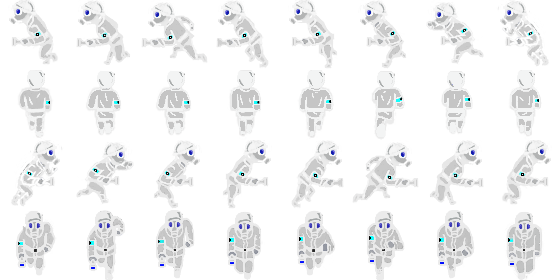
\includegraphics[keepaspectratio=true,scale=2]{images/ghostGuarda.png}
\end{figure}

\subsection{O boss do game}
O boss do game, o fantasma fuzilado, aparece na fase 5, última fase do jogo antes das fases bônus. Assim que o player pega a chave da quinta sala, um grito é ecoado na sala e ele surge. Ele é mais rápido que os demais fantasmas, causa mais dano que os demais fantasmas e atravessa as salas além de também ser invencível. Ao avistá-lo, o jogador deve usar todas as habilidades e experiências adquiridas até o momento para fugir do fantasma o mais rápido possível rumo à próxima fase.
\begin{figure}[h]
    \centering
    \caption{Imagem do Boss \textit{in game}}
     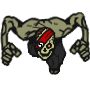
\includegraphics[keepaspectratio=true,scale=6]{images/bossf4.png}
\end{figure}

\section{Progresso do Jogo}
O progresso do jogo é contínuo e as fases podem ser mais rápidas ou demoradas de acordo com o fator randico dos itens.

A partir da fase 5, todas as fases serão fases bonus, o jogo continua enquanto o jogador tiver vidas.